\chapter{Collectivity in QCD}
\section{Conceptual Understanding of Collectivity and Flow}
The observation of collectivity in matter can be a powerful indicator of fundamental properties in that matter. Collectivity means many discrete structures are interacting together to form a whole. In high energy heavy ion physics, collectivity can be thought of as a medium formed that can be described as a locally equilibrated system evolving hydrodynamically instead of a group of individually interacting constituents. Collectivity is measured by looking for long-range angular correlations in the spray of final state particles that come out of the collision. A key property of high energy heavy ion collisions is that information on the initial conditions will be carried through the medium evolution. Thus, an asymmetry in the initial conditions of the heavy ion collision is measurable in the final products
\begin{figure}[!ht]
\begin{center}
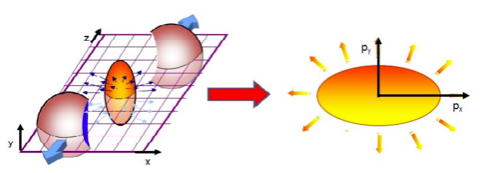
\includegraphics[width=0.45\linewidth]{figs/elliptical_flow_cartoon.png}
\caption{ The diagram demonstrating the relation between initial state geometry being transformed into final state momentum anisotropy. }
\end{center}
\end{figure}

\section{Mathematical Introduction}
A measurement of the azimuthal anisotropy is a way to quantify the extent of long-range angular correlation present in the medium evolution. Features of azimuthal anisotropy can be studied by creating a correlation function. The 2-particle correlation function method uses pairs of particles from the event in order to create a correlation function. For each each pair in an event, a $\Delta\phi$ value is obtained which makes up the signal $S(\Delta\phi,p_T)$. In order to correct for artificial correlations which would distort the distribution from detector effects or other sources, a mixed event background distribution $M(\Delta\phi,pT)$ is created. The correlation function can be defined as follows:

%\begin{equation}\label{eqn:corr_func}
 %C(\Delta,p_T) = \frac{S(\Delta\phi,p_T)}{M(\Delta\phi,p_T)}\frac{\int_{0}^{2\pi}M(\Delta\phi,p_T)d\Delta\phi)}{\int_0^{2\pi}S(\Delta\phi,p_T)d\Delta\phi)}
%\end{equation}

%multi particle cumulants - later
%correlation function
%describe c2 vs v2

\begin{eqnarray}
  \textbf{q} \cos(\Psi_R) = \frac{\textbf{Q}}{\sqrt{N}} = \sum^N_{j=1} \cos(\phi_j), & &
  \textbf{q} \sin(\Psi_R) = \frac{\textbf{Q}}{\sqrt{N}} = \sum^N_{j=1} \sin(\phi_j), 
\end{eqnarray}

\begin{eqnarray}
  S(\Delta\phi,p_{T})=
  \frac{ N^{{\rm track}(p_{T}){\rm }}_{{\rm Same \; event}}) }{ d\Delta\phi}, & &
\label{eq31} \\
  C(\Delta\phi,p_{T}) =
          \frac{S(\Delta\phi,p_{T})}{M(\Delta\phi,p_{T})} \:
          \frac{\int_{0}^{2\pi} M(\Delta\phi,p_{T}) \, d\Delta\phi}{\int_{0}^{2\pi} S(\Delta\phi,p_{T}) \, d\Delta\phi}. & &
  \label{eq:def_corr_function}
\end{eqnarray}

Substantial variations in this $C(\Delta\phi,p_T)$ are usually seen as long-range angular correlations which can be attributed to collectivity.

Another mathematical treatment regarding q-vectors is given: 

\begin{eqnarray}
  \textbf{q} \cos(\Psi_R) = \frac{\textbf{Q}}{\sqrt{N}} = \sum^N_{j=1} \cos(\phi_j), & &
  \textbf{q} \sin(\Psi_R) = \frac{\textbf{Q}}{\sqrt{N}} = \sum^N_{j=1} \sin(\phi_j), 
\end{eqnarray}

where $|q| \geq 0$.

\begin{equation}
  \sigma_\nu^2 \equiv \left<\nu^2\right> - \left<\nu\right>^2.
\end{equation}

\begin{figure}[!ht]
\begin{center}
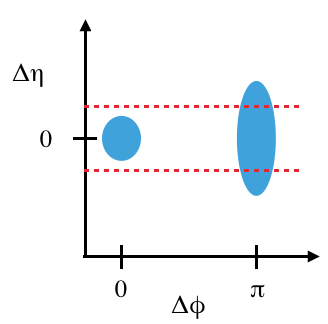
\includegraphics[width=0.45\linewidth]{figs/jet_corr_example.png}
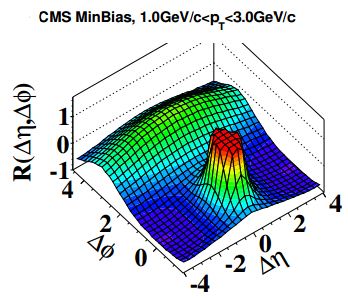
\includegraphics[width=0.47\linewidth]{figs/pp_correlation_function_min_bias.png}
\caption{Plotted here is the 2D profile of a correlation function in $\Delta\eta \Delta\phi$ space of a dijet event. The red dotted lines represent the exclusion zone in $\Delta\eta$ where to  make the measurement to reduce non-flow contributions.}
\label{fig:jet_corr_example}
\end{center}
\end{figure}

In order to quantify the azimuthal anisotropy, $C(\Delta\phi,p_T)$ is Fourier transformed:
\begin{equation}\label{eqn:dndphi}
  C(\Delta\phi,p_T) \propto 1 + \sum_{n=1}2 v_{n}\cos(n[\phi(p_T)-\Psi_n]) 
\end{equation}

where $\Psi_n$ is the event plane angle, $\phi$ is the azimuth of tracks from the event, and $v_n$ are flow coefficients. The measured $v_n$ averaged over a single event is defined as:
\begin{equation}\label{eqn:vn}
  v_n = \frac{\langle\cos(n[\phi-\Psi_n])\rangle}{Res(\Psi_n)}
\end{equation}

where $Res(\Psi_n)$ is the event plane resolution for each event. $v_N$ are further averaged over each event.
\begin{equation}
\varepsilon_n = \frac{\sqrt{\langle r^2\cos (n\phi)\rangle ^2 + \langle r^2\sin (n\phi) \rangle ^2}}{\langle r^2 \rangle}
\end{equation}

%\begin{figure}[h!]
%\begin{center}
%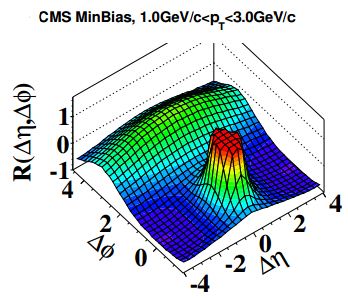
\includegraphics[width=0.45\linewidth]{figs/pp_correlation_function_min_bias.png}
%\caption{ }
%\label{fig:pp_corr_func_minbias}
%\end{center}
%\end{figure}

The significance of a the so called ``near-side ridge" is due to the fact that region in $\Delta\phi$, $\Delta\eta$ space can only be comprised of pairs of particles with long range angular correlations unassociated with any known non-flow effects.

\section{A Review of Flow Measurements in Small Collision Systems}
%p+p ridge
%he3au v3
%pPb
%other experiments
% mass ordering

As mentioned at the end of Chapter 1, small collision systems have been considered too small to create hot and dense matter. These systems were used as control experiments which could be used to measure how the presence of a nucleus would effect the production of particles relative to $p+p$ collisions. These so called "cold nuclear matter" (CNM) effects would be isolated when colliding very low $Z$ nuclei, such as a deuteron or proton, with a large nucleus.\footnote{ A quick side note: the convention in the field of heavy ion physics is to label any such small system collisions as $p$+A and any large system collisions as A+A} Generally accepted CNM effects are: nuclear shadowing which is the modification of parton distribution functions by a nucleus, gluon saturation, radiative energy loss which is the modification of the momentum fraction of partons due to multiple soft scatterings, and finally the Cronin effect which is the broadening of the transverse momentum of emitted particles distribution due to multiple scatterings of initially colliding partons \textbf{add ref}.  

%\subsection{Nearside Ridge in Small Systems}
In 2010, the CMS collaboration published a paper observing a nearside ridge in high multiplicity 7 TeV $p+p$ events in the two-particle correlation function for dihadrons as shown in Figure \ref{fig:pp_ridge_plot}. The aforementioned nearside ridge is located at $\Delta\phi$ = 0 and at $|\Delta\eta| > $ 2 in the figure. The ridge is significant in contrast to the minimum bias $p+p$ correlation function shown in Figure \ref{fig:pp_corr_func_minbias} with an absence of any such ridge.
\begin{figure}[h!]
\begin{center}
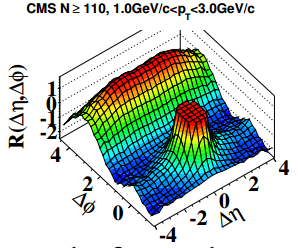
\includegraphics[width=0.55\linewidth]{figs/pp_high_multiplicity_ridge.PNG}
\caption{ 2-D two-particle correlation function for $p+p$ collisions at \sqsn = 7 TeV for hadrons with 1.0 $<|p_T|<$ 3.0 GeV/c in high multiplicity events with greater than 109 charged particle tracks were found \cite{Khachatryan2010}.}
\label{fig:pp_ridge_plot}
\end{center}
\end{figure}

What this discovery showed was that collectivity-like effects could be measured in small collisions systems for high-multiplicity events. Thus, $p+Pb$ at \sqsn = 5.02 TeV events were analyzed to find flow. A nearside ridge was observed in 0-20\% central events What became apparent over the course of making such measurements is that the non-flow contribution to the signal would be much larger for p+A events then that of A+A events. Schemes were developed to reduce the non-flow component in the flow measurement. Figure \ref{fig:pPb_ridge_subtraction} demonstrates one such scheme. The idea is to measure the same two-particle correlation function for central, high-multiplicity, events and for peripheral events, in this case 0-20\% central and 60-100\% central and then subtract the central correlation function by the peripheral one. The assumption being that the level and shape of the non-flow is mostly consistent across centrality classes whereas the flow is very centrality dependent such that there is virtually no flow in the peripheral correlation function. Thus, by subtracting the central correlation function by the peripheral, only the like components to both will be subtracted out, which are the non-flow components. As seen in panel three in Figure \ref{fig:pPb_ridge_subtraction}, the subtracted correlation function has no dominating jet peak at (0,0) and the nearside and awayside ridges are distinct and clear.

\begin{figure}[h!]
\begin{center}
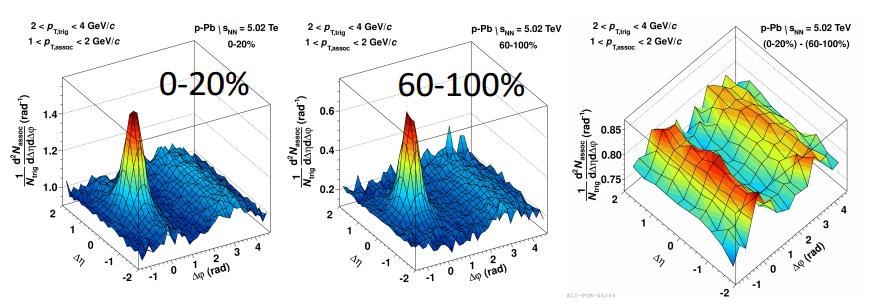
\includegraphics[width=0.85\linewidth]{figs/pPb_subtraction_correlation.PNG}
\caption{ 2-D two-particle dihadron correlation function for $p+Pb$ collisions for 0-20\% and 60-100\% centrality events as measured by the ALICE detector in the left and middle panel, respectively. The rightmost panel shows the subtraction of the left panel by the middle panel to remove background. [?]}
\label{fig:pPb_ridge_subtraction}
\end{center}
\end{figure}

%\subsection{Mass Ordering in $v_2$}
A key observation in the determination of real collective flow is a mass ordering in the strength of the flow coefficients. The left panel of Figure \ref{fig:PbpPb_mass_ordering} depicts the observed mass ordering of particles in Pb+Pb 10-20\% centrality events. In the low $p_T$ region of 0 - 2 GeV, the magnitude of $v_2$ for hadrons, going from largest to smallest, is $\pi^{\pm}$, $K^{\pm}$, and $p+pbar$ and other heavier particles, which is the same order as the particles mass's (reword this sentence). The mass ordering effect can be thought of as primarily reduction in the $v_2$ for low $p_T$ heavy hadrons. Assuming an elliptic flow is present, the steep pressure gradients will efficiently modify the magnitude of $p_T$ for heavy hadrons more than for light hadrons which leads to a reduction in the number of heavy hadrons available at low $p_T$ to produce a low $p_T$ $v_2$ \cite{PhysRevC.77.044909}. Thus, the mass ordering observation is taken to be evidence that the system is creating a medium such that particles will flow in predictable ways.

\begin{figure}[h!]
\begin{center}
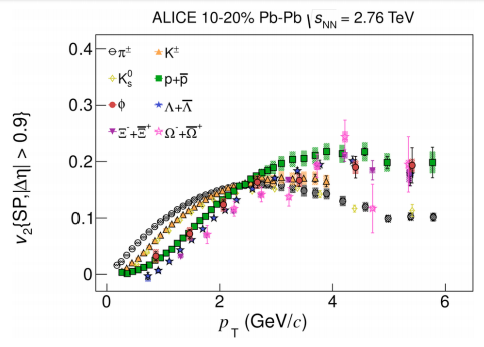
\includegraphics[width=0.48\linewidth]{figs/PbPb_v2_mass_ordering.PNG}
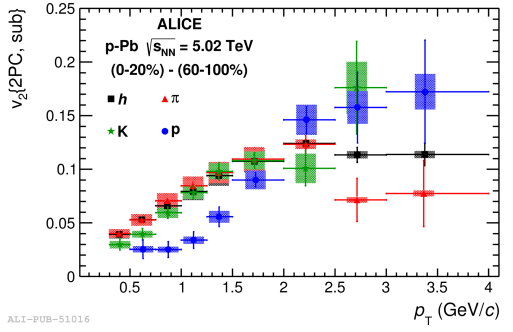
\includegraphics[width=0.48\linewidth]{figs/pPb_two_part_v2_mass_ordering.PNG}
\caption{$v_2(p_T)$ for different particles in Pb-Pb \sqsn = 2.76 TeV 10-20\% events as measured by the ALICE detector. The $\Delta\eta$ gap at minimum is 0.9 units. The right plot shows the $v_2(p_T$ for different particles in p-Pb \sqsn = 5.02 TeV for 0-20\% events that were subtracted by peripheral 60-100\% events. The $v_2$ is extracted directly from the two particle correlation function shown in Figure \ref{fig:pPb_ridge_subtraction}. \textbf{add refs}}
\label{fig:PbpPb_mass_ordering}
\end{center}
\end{figure}

The right panel of Figure \ref{fig:PbpPb_mass_ordering} shows a similar plot to the left panel of that figure except for the system $p+Pb$ \sqsn = 5.02 TeV. As in the $Pb+Pb$ system, a noticeable mass ordering is observed. The order is the same as in the $Pb+Pb$ as well as the shapes of each $v_2(p_T)$ curve. Thus, mass ordering is observed is small systems such as pA as well as AA. An important note for the result on the right panel is that a central minus peripheral subtraction was done, as demonstrated in Figure \ref{fig:pPb_ridge_subtraction} whereas the result in the left panel needed no such peripheral subtraction. This means it is difficult to compare directly with the A+A result in magnitude, although the similarity of the ordering and the shape of the curves is enough of a comparison to indicate collectivity in the small system.
%\begin{figure}[h!]
%\begin{center}
%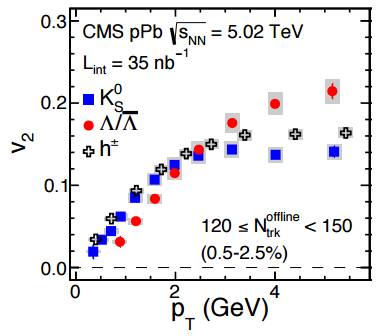
\includegraphics[width=0.55\linewidth]{figs/pBp_v2_mass_ordering.PNG}
%\caption{ CMS The correlation function for $p+p$ collisions at \sqsn = 7 TeV for hadrons with 1.0 $<|p_T|<$ 3.0 GeV/c in high multiplicity events with greater than 109 charged particle tracks were found \cite{Khachatryan2010}.}
%\label{fig:pp_ridge_plot}
%\end{center}
%\end{figure}

Flow measurements in small systems have also be made at a lower energy accelerator. 

\begin{figure}[h!]
\begin{center}
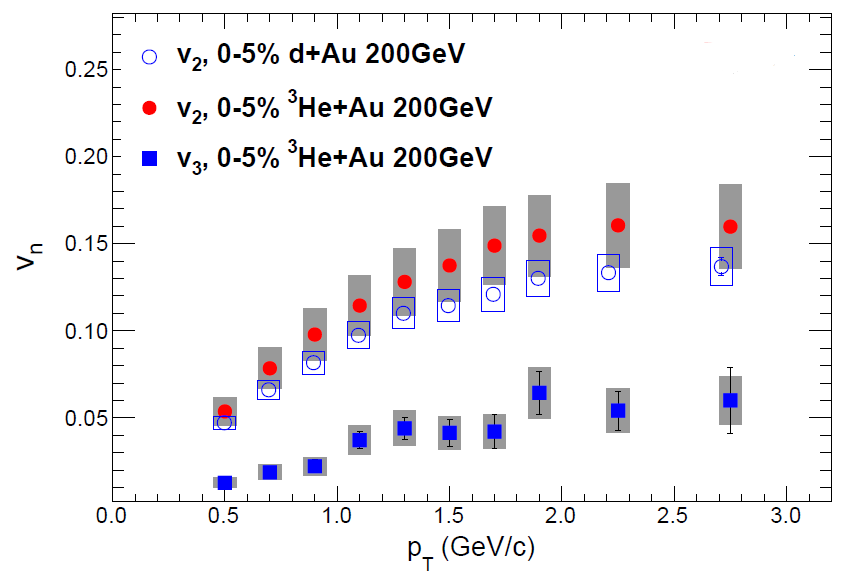
\includegraphics[width=0.75\linewidth]{figs/hedau_v2_v3.PNG}
\caption{ The correlation function for $p+p$ collisions at \sqsn = 7 TeV for hadrons with 1.0 $<|p_T|<$ 3.0 GeV/c in high multiplicity events with greater than 109 charged particle tracks were found \cite{Khachatryan2010}.}
\label{fig:pp_ridge_plot}
\end{center}
\end{figure}

\begin{figure}[h!]
\begin{center}
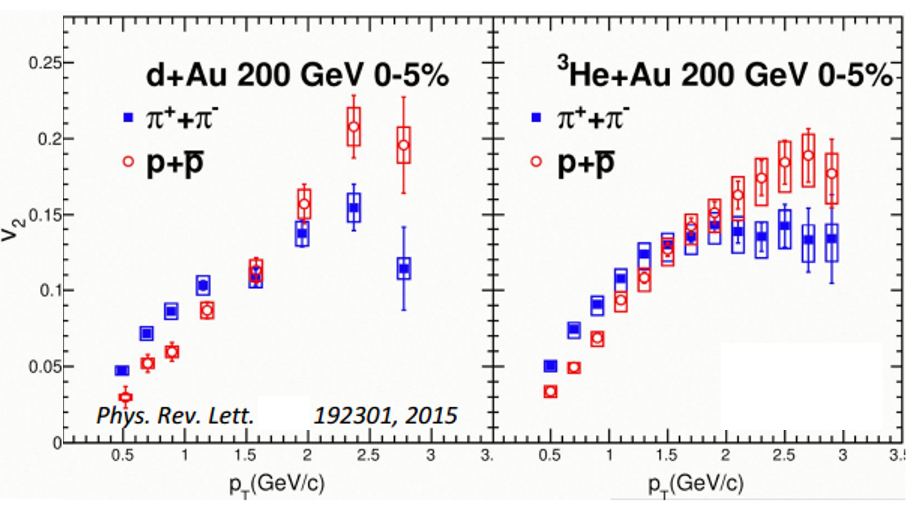
\includegraphics[width=0.65\linewidth]{figs/dhau_mass_ordering_phenix.PNG}
\caption{ The correlation function for $p+p$ collisions at \sqsn = 7 TeV for hadrons with 1.0 $<|p_T|<$ 3.0 GeV/c in high multiplicity events with greater than 109 charged particle tracks were found \cite{Khachatryan2010}.}
\label{fig:pp_ridge_plot}
\end{center}
\end{figure}

\begin{figure}[h!]
\begin{center}
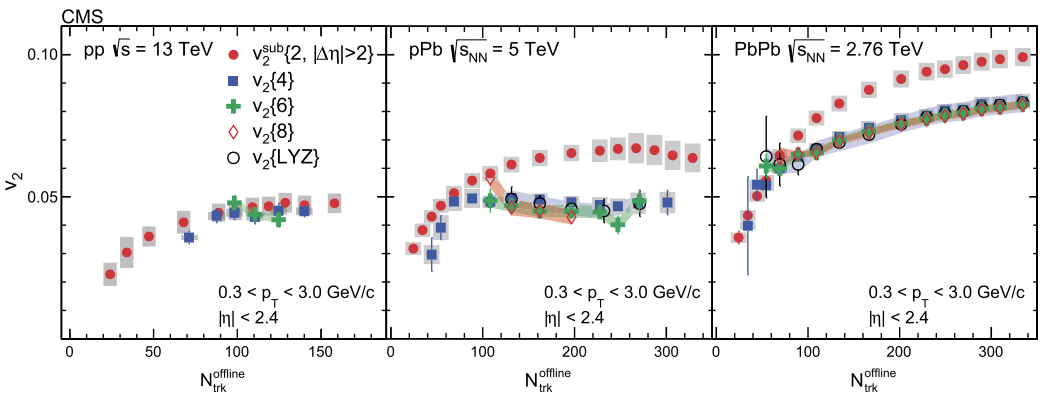
\includegraphics[width=0.9\linewidth]{figs/pp_pPb_PbPb_cumulants.PNG}
\caption{ The correlation function for $p+p$ collisions at \sqsn = 7 TeV for hadrons with 1.0 $<|p_T|<$ 3.0 GeV/c in high multiplicity events with greater than 109 charged particle tracks were found \cite{Khachatryan2010}.}
\label{fig:pp_ridge_plot}
\end{center}
\end{figure}


%paul romatchke ryan, 3 panel plot constituent quark initial condition pp 
% 6-8 and Lee Yang zeros N-body correlation, not a two body decay that correlations particles, not back to back jets correlated because tehy all feel the effects the initial geometry

A caveat to all these measurements is that throughout the whole process of small systems being considered as possible producers of a thermally equilibrated medium, there is alternative explanations to explain the apparent flow measured in small systems which do not involve the creation of a medium. In order to contribute to the distinction between a medium and a non-medium explanation, three different small collision systems each with unique initial conditions were run at RHIC. Those three systems are d+Au, He+Au, and finally p+Au, with built in elliptical, triangular, and circular geometric initial conditions. The constraints that a set of measurements from all three systems would place upon explanatory models would help distinguish which described small systems best. The thesis is a completion of that set of three measurements, by measuring the p+Au dataset. 


%However, evidence of collectivity has recently been observed at RHIC in p+Au collisions at $\sqrt{s_{NN}}$ = 200 GeV in the most central collisions ~\cite{PhysRevLett.115.142301}. Although, the $p_T$ dependent $v_N$ has been measured, what has not been measured in these small systems is the degree to which $v_N$ changes a function of rapidity. This is a particularly interesting measurement to make in an asymmetric collision system such as p+Au.

%Recent analyses of d+Au and HeAu collisions at $\sqrt{n}$ = 200 GeV~\cite{PhysRevLett.111.212301,Adare:2014keg,Adare:2015ctn,Adamczyk:2014fcx} at the Relativistic Heavy-Ion Collider (RHIC), and p+Pb at $\sqrt{n}$ = 5.02 TeV, and $p+p$ collisions at $\sqrt{n}$ = 2.76, 5.02, 7, and 13 TeV~\cite{alice_long_2013,atlas_observation_2012,cms_observation_2012,Khachatryan:2015lva,Aad:2015gqa,Khachatryan:2010gv,Khachatryan:2016txc} at the Large Hadron Collider (LHC) have demonstrated the existence of the same kind of azimuthal anisotropy signals commonly interpreted as evidence of collective behavior in larger systems. Notably, a feature known as \textit{the ridge} has been observed, consisting of a near-side (i.e., at small relative azimuth) enhancement in the long-range (i.e., at large relative pseudorapidity) azimuthal two-particle correlation. From these correlations, substantial elliptic ($v_2$), and triangular ($v_3$) flow coefficients have been measured in these systems.

%\iffalse

\section{An Overview of Simulations}

\subsection{Initial Condition}
\subsubsection{Monte-Carlo Initial Condition Characterization}
\begin{figure}[h!]
\begin{center}
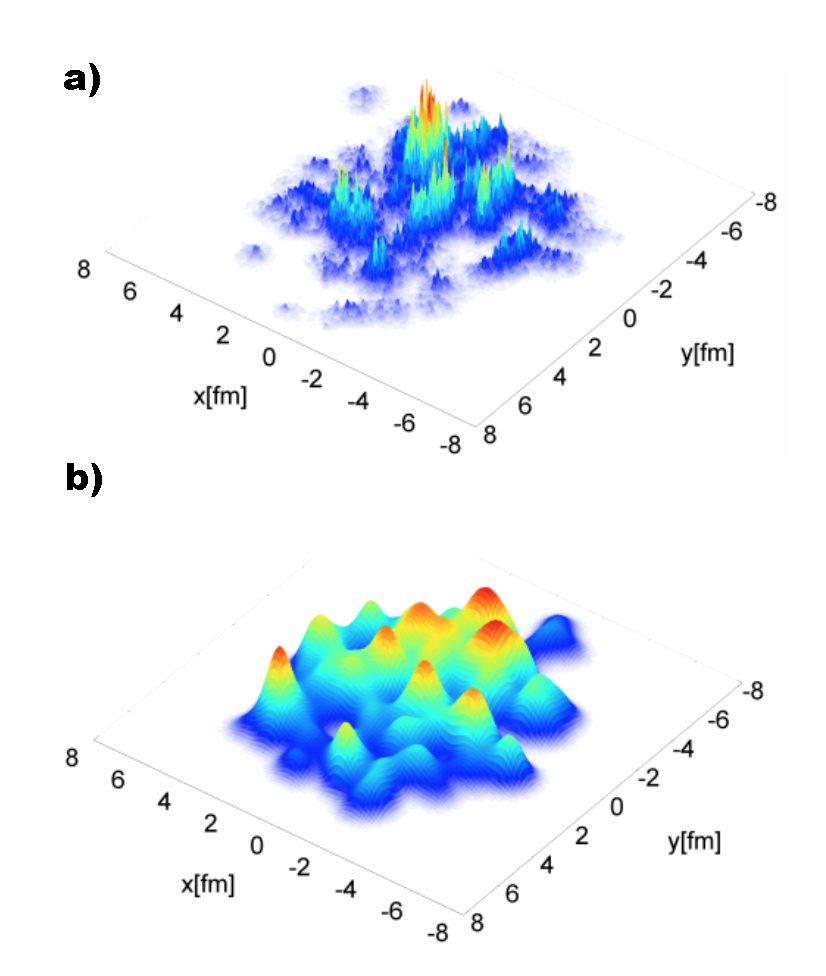
\includegraphics[width=0.45\linewidth]{figs/initial_conditions.png}
\caption{ a) IP-glasma. b) MC-KLN. c) MC-Glauber.}
\end{center}
\end{figure}

\begin{figure}[h!]
\begin{center}
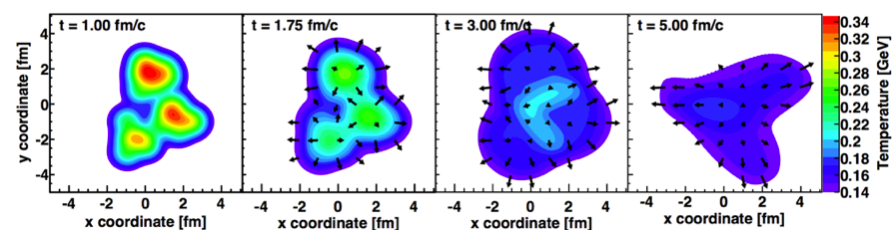
\includegraphics[width=0.45\linewidth]{figs/he3au_simulation.png}
\caption{ TBA }
\end{center}
\end{figure}

\subsubsection{IP Glasma}

\subsection{Hydrodynamic Treatment}

\subsubsection{SONIC}

\subsubsection{SuperSONIC}

\subsection{AMPT}

%\fi